\chapter{Live Mode}
\label{sec:live_mode}

There exist 3 application modes:
\begin{itemize}
\item 'Offline': Default mode, for offline analysis
\item 'Live: Running': Provides a live display of network data, while also importing the ASTERIX data into the database
\item 'Live: Paused': Provides offline-like analysis, which caching ASTERIX network data and allows resuming into 'Live: Running' without loss of data
\end{itemize}
\ \\

\begin{figure}[H]
 \center
    
\includegraphics[width=8cm]{figures/modes.png}
  \caption{Application Modes}
\end{figure}


The application switches in Live mode when ASTERIX data is imported from the network, as described in \nameref{sec:ui_import_asterix_network}. \\

The data sources network lines have to be defined in as described in \nameref{sec:configure_datasources_table_content}. \\

When that Live mode is enabled and the correct network lines are setup (and active) the main window is shown as follows. 

\begin{figure}[H]
  \hspace*{-2.5cm}
    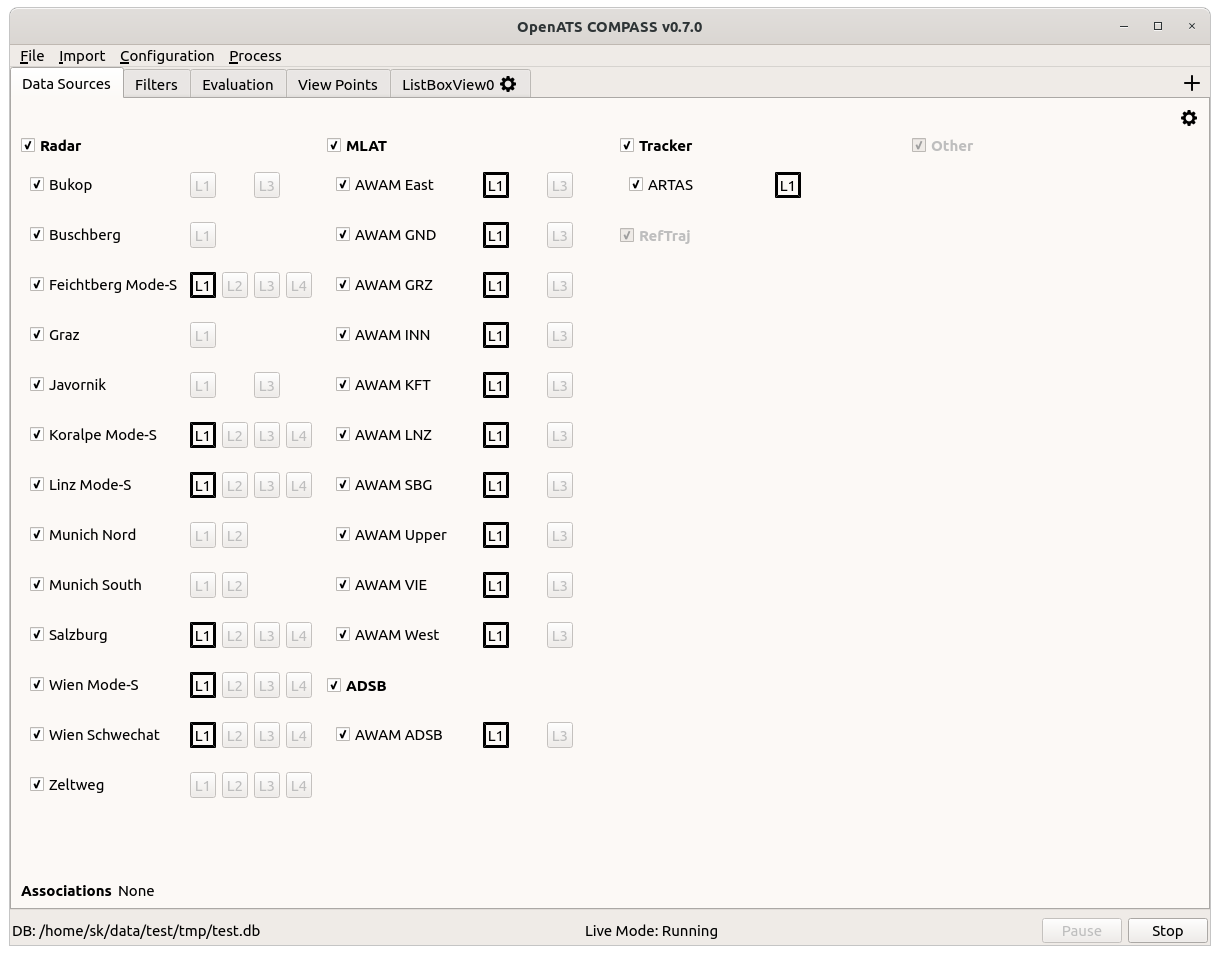
\includegraphics[width=19cm]{figures/live_mode.png}
  \caption{Main Window in Live Mode}
\end{figure}

In Live mode, most application components are the same as in Offline mode (although some are deactivated), but in the main status bar the Live mode is indicated. Using the 'Pause' button the 'Live: Paused' mode can be entered and the 'Stop' button allows stopping the network recording and returning to Offline mode.

\section{Data Sources \& Processing}

For each data source, the defined lines are shown (as L1 ... L4 buttons). If no data is received (on a define Line), the respective button is disabled (greyed out). If data is received over a line, it will be come active and the received data stored in the database. If a update interval is specified for the respective data source, the line button background color will become green in current data was received during the last 2 update intervals. \\

The line button can also be toggled - if a bold border is shown the data from the respective line stored not only in the database but \textbf{also} in main memory (RAM). The most recent 5 minutes of data are kept in main memory (RAM), and can be visualized in the existing Views. \\

Please \textbf{note} that currently only the OSG View displays data in live mode, for performance reasons the other Views are inactive.

\section{OSG View}

In Live mode, the OSG View automatically shows the same elements as with the time filter, and the main components are the same as in Offline mode (although some are deactivated).

\begin{figure}[H]
    \hspace*{-2.5cm}
    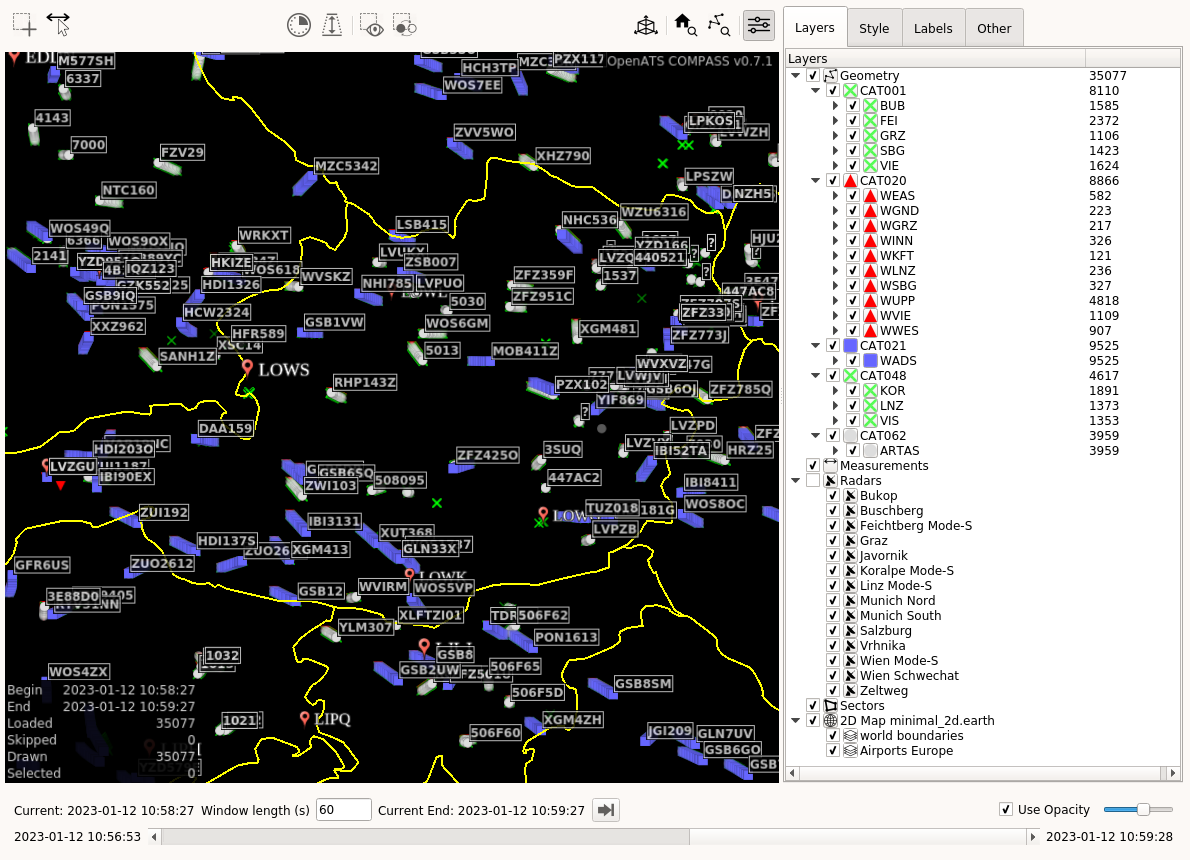
\includegraphics[width=19cm,frame]{figures/osg_live_mode.png}
  \caption{OSG View in Live Mode}
\end{figure} 

In the time filter elements, at maximum 5 minutes of past data is available. In a 1 second update newly received network data is shown, and the labels updated (if automatic labeling is enabled). \\

Using the time scrollbar, past data can be inspected, which is kept until it becomes outdated (older than 5 minutes) or the scrollbar is moved to the most right position. In this position, the displayed time window will again follow the most recent time.




